\section {Один корень внутри промежутка}

Так же, как и в первом случае, здесь возможны четыре типа границ. Напомним их:

\begin {enumerate} [labelindent=\parindent, leftmargin=*]
    \item {$[\alpha, \beta]$}
    \item {$[\alpha, \beta)$}
    \item {$(\alpha, \beta]$}
    \item {$(\alpha, \beta)$}
\end {enumerate}

Для типов границ 1--3 возможны два особых случая:

\begin {itemize}
    \item {существует два корня, при этом один из них попадает на включённую границу промежутка, а
           второй "--- за его пределы}
    \item {существует два корня, при этом один из них попадает на выколотую границу промежутка, а
           второй "--- на промежуток}
    \item {существует ровно один корень, который попадает внутрь промежутка}
\end {itemize}

\subsection {Границы 2 типа}

Особым случаям 2 типа границ будет соответствовать следующие ситуации:

\begin {figure} [h]
    \begin {minipage} [t] {0.3\linewidth}
        \centering
        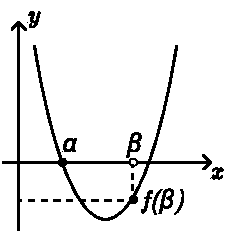
\includegraphics [width=\linewidth] {images/image_03.pdf}
    \end {minipage}
    \hfill
    \begin {minipage} [t] {0.3\linewidth}
        \centering
        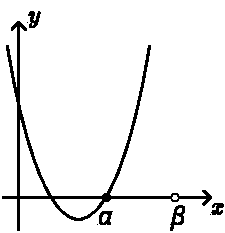
\includegraphics [width=\linewidth] {images/image_17.pdf}
    \end {minipage}
    \hfill
    \begin {minipage} [t] {0.3\linewidth}
        \centering
        \includegraphics [width=\linewidth] {images/image_04.pdf}
    \end {minipage}
\end {figure}

\subsubsection {Первый особый случай}
Чтобы обработать первый случай, нужно рассмотреть прохождение параболы $y = f(x)$ через точку
$x = \alpha$. То есть решить уравнение

\begin {equation*}
    f(\alpha) = 0
\end {equation*}

Далее, подставить полученные значения параметра $p$ в трёхчлен $f(x)$ и выбрать параметры, при
которых второй корень существует и лежит за пределами промежутка $[\alpha, \beta)$. Это можно
сделать с помощью теоремы Виета или проверки соответствующего условия:

\begin {equation*}
    a \cdot f(\beta) \leqslant 0
\end {equation*}

\subsubsection {Второй особый случай}
Во втором случае нужно рассмотреть прохождение параболы через выколотую точку $x = \beta$:

\begin {equation*}
    f(\beta) = 0
\end {equation*}

Далее, подставить полученные значения параметра $p$ в трёхчлен $f(x)$ и выбрать параметры, при
которых второй корень существует и лежит внутри промежутка $[\alpha, \beta)$. Это можно
сделать с помощью теоремы Виета или проверки соответствующих условий:

\begin {equation*}
    \begin {cases}
        D > 0,
        \\
        a \cdot f(\alpha) \geqslant 0,
        \\
        \alpha \leqslant x_0 < \beta.
    \end {cases}
\end {equation*}

\subsubsection {Третий особый случай}

Чтобы обработать третий случай, нужно рассмотреть равенство дискриминанта нулю, а потом
подставить полученные значения параметра $p$ в трёхчлен $f(x)$ и выбрать параметры, при которых
$x_0$ лежит внутри промежутка $[\alpha, \beta)$. Это можно сделать с помощью проверки условий:

\begin {equation*}
    \alpha \leqslant x_0 < \beta
\end {equation*}

\subsection {Границы 4 типа. Общий случай}

Для границ 4 типа существует три особых случая, которые описаны выше. В данном пункте на примере
этих границ мы разберем общий случай:

\begin {figure} [h]
    \begin {minipage} [t] {\linewidth}
        \centering
        \includegraphics [width=0.3\linewidth] {images/image_05.pdf}
    \end {minipage}
\end {figure}

Чтобы ровно один корень был внутри интервала $(\alpha, \beta)$ необходимо существование двух корней,
положительное значение трёхчлена $f(x)$ на одном конце и отрицательное на другом. Получаем
следующую совокупность двух систем:

\begin {equation*}
    \left[
        \begin {gathered}
            \begin {cases}
                a \cdot f(\alpha) < 0
                \\
                a \cdot f(\beta) > 0
            \end {cases}
            \\
            \begin {cases}
                a \cdot f(\alpha) > 0
                \\
                a \cdot f(\beta) < 0
            \end {cases}
        \end {gathered}
    \right.
\end {equation*}

Как уже говорилось, чтобы получить полное решение задачи, нужно объединить особые случаи с общим
случаем.
